\documentclass{article} % For LaTeX2e

\usepackage{nips13submit_e,times}
%\usepackage{hyperref}
\usepackage{url}
\usepackage{array}
\usepackage{amsmath,amssymb} % define this before the line numbering.
\usepackage{subfigure}
%\usepackage{subcaption}

\usepackage[breaklinks=true,letterpaper=true,colorlinks,bookmarks=false]{hyperref}

\usepackage{graphicx} % more modern

%\usepackage{epsfig} % less modern

% For citations
%\usepackage{natbib}

% For algorithms
\usepackage{algorithm}
\usepackage{algorithmic}

\usepackage{amsmath,amssymb} 
\usepackage{makecell}
\usepackage{booktabs}

\usepackage{helvet}
\usepackage{courier}
\usepackage{hyperref}


\newtheorem{theorem}{Theorem}
\newtheorem{lemma}{Lemma}
\newtheorem{proposition}{Proposition}
\newtheorem{corollary}{Corollary}
\newtheorem{assumption}{Assumption}
%\newtheorem{remark}{Remark}

\newcommand{\argmax}{\mathop\mathrm{argmax}}
\newcommand{\argmin}{\mathop\mathrm{argmin}}


\newenvironment{proof}[1][Proof]{\begin{trivlist}
\item[\hskip \labelsep {\bfseries #1}]}{\end{trivlist}}
\newenvironment{definition}[1][Definition]{\begin{trivlist}
\item[\hskip \labelsep {\bfseries #1}]}{\end{trivlist}}
\newenvironment{example}[1][Example]{\begin{trivlist}
\item[\hskip \labelsep {\bfseries #1}]}{\end{trivlist}}
\newenvironment{remark}[1][Remark]{\begin{trivlist}
\item[\hskip \labelsep {\bfseries #1}]}{\end{trivlist}}
\newcommand{\qed}{\nobreak \ifvmode \relax \else
      \ifdim\lastskip<1.5em \hskip-\lastskip
      \hskip1.5em plus0em minus0.5em \fi \nobreak
      \vrule height0.75em width0.5em depth0.25em\fi}

\renewcommand{\theHalgorithm}{\arabic{algorithm}}
\renewcommand{\algorithmicrequire}{\textbf{Input:}}
\renewcommand{\algorithmicensure}{\textbf{Output:}}
\newcommand{\SWITCH}[1]{\STATE \textbf{switch} (#1)}
\newcommand{\ENDSWITCH}{\STATE \textbf{end switch}}
\newcommand{\CASE}[1]{\STATE \textbf{case} #1\textbf{:} \begin{ALC@g}}
\newcommand{\ENDCASE}{\end{ALC@g}}
\newcommand{\CASELINE}[1]{\STATE \textbf{case} #1\textbf{:} }
\newcommand{\DEFAULT}{\STATE \textbf{default:} \begin{ALC@g}}
\newcommand{\ENDDEFAULT}{\end{ALC@g}}
\newcommand{\DEFAULTLINE}[1]{\STATE \textbf{default:} }


\title{Stochastic Optimization of Black-box Functions on Riemannian Manifolds Using Kernel Adaptive SMC}


\author{
Hanchen Xiong \quad Sandor Szedmak \quad Phillip Zech \quad Justus Piater 
%\thanks{ Use footnote for providing further information
%about author (webpage, alternative address)---\emph{not} for acknowledging
%funding agencies.} 
\\
Institute of Computer Science \\
University of Innsbruck\\
Technikerstr.21a, Innsbruck, A-6020, Austria \\
\textit{\{hanchen.xiong, sandor.szedmak, phillip.zech, justus.piater\}@uibk.ac.at} \\
%\And
%Coauthor \\
%Affiliation \\
%Address \\
%\texttt{email} \\
%\AND
%Coauthor \\
%Affiliation \\
%Address \\
%\texttt{email} \\
%\And
%Coauthor \\
%Affiliation \\
%Address \\
%\texttt{email} \\
%\And
%Coauthor \\
%Affiliation \\
%Address \\
%\texttt{email} \\
%(if needed)\\
}

% The \author macro works with any number of authors. There are two commands
% used to separate the names and addresses of multiple authors: \And and \AND.
%
% Using \And between authors leaves it to \LaTeX{} to determine where to break
% the lines. Using \AND forces a linebreak at that point. So, if \LaTeX{}
% puts 3 of 4 authors names on the first line, and the last on the second
% line, try using \AND instead of \And before the third author name.

\newcommand{\fix}{\marginpar{FIX}}
\newcommand{\new}{\marginpar{NEW}}

\nipsfinalcopy % Uncomment for camera-ready version

\begin{document}

\maketitle

\begin{abstract}
This paper puts forward a new stochastic method for global optimization of black-box functions on a Riemannien manifold $\mathcal{M}$,   
which is rather challenging yet useful in many areas. The proposed algorithm is based on \emph{Kernel Adaptive Sequential 
Monte Carlo} (KASMC) by exploiting the closeness between simulated annealing and sequential Monte Carlo (SMC), and thus is referred to as KASMC optimizer.             
At each Markov chain Monte Carlo (MCMC) transition of KASMC optimizer, samples are first proposed in a reproducing kernel Hilbert space (RKHS) of the embeding space 
of $\mathcal{M}$, after adaptively tempered acceptance criterion, they are mapped back to the embeding space and $\mathcal{M}$ respectively by two projection steps.     
The strength of KASMC optimizer, compared to classical simulated annealing, stems from its two adaptive  
tunning mechanisms. The first one is adaptive tempering, which automatically constructs temperature schedule through cooling; 
the second one is adaptive MCMC transition in RKHS, which is 
critical to fit highly nonlinear support of functions. 
%Therefore, KASMC is fully adaptive and no parameter tuning is needed.
Furthermore, a finite-time performance guarantee of KASMC optimizer is provided.   
Based on our experimental results on $SO(3)$ manifold and Stiefel manifold, KASMC demonstrates promising applicabilities.     
\end{abstract}

\section{Introduction}
Global optimization on a black-box function $f$ is a long-standing challenge task  
despite its wide usage and demand in many disciplines \cite{black_box_optimization, black_box_optimization_book}.    
Difficulties are usually considered from two aspects: \emph{i.} the analytic form of $f$ is unknown and function values can 
be only accessed point-wisely, thus no function landscape property (\emph{e.g.} convexity or local convexity) can be exploited for numerical solutions;     
%\emph{ii}. function evaluation is usually at high cost, which narrows algorithms to be practical only if they can find 
%optima (with tolerant imprecision) under an affordable iteration budget. 
\emph{ii.} the function can be arbitrarily complex, \emph{e.g.} high-dimensional, multi-modal, which tends to trap solutions in local optimum. 
In this paper, we consider an even more ``nasty" case, where 
$f$ is defined on a Riemannien manifold $\mathcal{M}$ (see Figure \ref{fig:overview}). Since the support of $f$ is $\mathcal{M}$ instead of $\mathbb{R}^d$, search     
should be more careful with exploration and exploitation restricted on $\mathcal{M}$.       
Very often the shape of $\mathcal{M}$ is irregular, which worsens the situation.       
However, this task arises in many areas \cite{SA_registration, Geo_MCMC}. 
Therefore, it is rather desirable to come up with a general algorithm which can at the best efficiency find good solutions with guaranteed 
precision. 

\emph{Simulated annealing} (SA) is a classical stochastic optimization method for black-box functions \cite{SA}. 
Experience users usually spend much effort in tuning parameters in SA to accelerate its convergence. 
Although an adaptive mechanism was introduced by Ingber (1996) \cite{ASA}, yet its applicability is restricted within
%only rescaling Guassian (co)variances in 
\emph{random walk metropolis algorithm}. 
Therefore, its adaptivity is rather limited for complex functions.     
%Also, a theoretic analysis of its convergence property is lacking. 
%However, its applicability is limited to common case where $f$ is defined on $\mathbb{R}^d$. 
In present paper, we propose an adaptive stochastic method to 
%extend simulated annealing to 
handle $f$ on Remannian manifolds. 
The proposed algorithm is based on \emph{Kernel Adaptive Sequential Monte Carlo}     
(KASMC) by exploiting the close analogy between SA and sequential Monte Carlo (SMC), and therefore is referred to as KASCM optimizer.    
Similar to SA, KASMC optimizer increases the determinism of proposal acceptance criterion by monotonically decreasing a temperature parameter.     
However, in KASMC, sequential tempering is implemented in a SMC instead, which can be considered as a multi-particle simulated annealing \cite{multi_particle_SA} 
with weighting and resampling.      
At each Markov chain Monte Carlo (MCMC) transition in the SMC, samples are first proposed in a \emph{reproducing kernel Hilbert space} (RKHS) of the embedding space  
of $\mathcal{M}$, after adaptively tempered acceptance criterion, they are mapped back to the embedding space and $\mathcal{M}$ respectively by two projection steps.     
The adaptive proposal construction in RKHS is inspired by \emph{MCMC Kameleon} \cite{MCMC_Kameleon}. Meanwhile, we improve MCMC Kameleon with a more effective 
method for finding pre-images by exploiting local topology consistence between RKHS and the embedding space.      
The strength of KASMC optimizer stems from its two adaptive  
tunning mechanisms. The first one is adaptive tempering, which, based on \emph{effective sampling size} (ESS), automatically constructs temperature schedule 
through cooling; 
the second one is adaptive MCMC transition in RKHS, which is 
critical to handle highly nonlinear support of $f$. 
Furthermore, based on previous studies, which include the finite-time performance analysis of simulated annealing on continuous domains \cite{SA_finite_time_2, SA_finite_time}         
and convergence property of adaptive SMC \cite{convergence_ASMC}, 
we present a finite-time performance guarantee of KASMC optimizer.   
In our experiments, the proposed KASMC optimizer was evaluated on two practical tasks: rotation optimization on $SO(3)$ manifold for 3D registration and 
subspace optimization on Stiefel manifold for dimension reduction in classification. According to our empirical results, KASMC optimizer consistently 
outperforms SA and other non(or weaker)-adaptive counterparts.   

%\subsection{Related Work}
\paragraph{Related Work} \quad
KASMC optimizer can be related to many other work from different perspectives. The following provides a short summary of recent development of relevant study. 
\textbf{Global optimization of black-box functions.} A review of methods for global optimization of black-box functions  
can be found in 
\cite{black_box_optimization} or \cite{black_box_optimization_book}.   
Out of all work, \emph{Bayesian optimization} \cite{BO_tutorial,BO_NIPS} 
and \emph{Hierarchical optimistic optimization} \cite{optimistic}
are two research branches which have recently attracted particularly more attention.  
Bayesian optimization is a \emph{response surface method} with Gaussian process to interpolate  
the unknown function $f$. Hierarchical optimistic optimization is an application of \emph{optimism principle} on 
\emph{Monte Carlo tree search} (MCTS), which partitions search spaces hierarchical and conducts exploration and 
exploitation at different scales.
%A combination of these two techniques was proposed in \cite{Bam_SOO}. 
To the best of our knowledge, no work has been conducted for Bayesian optimization or optimistic optimization on Riemannian 
manifolds. Only one work on Bayesian optimization with constraints \cite{BO_constraint} can be, in some cases, extended to Reimannian manifolds.        
\textbf{Linking SA and SMC.} SA and SMC were rarely connected although both of them have been employed for stochastic optimization.  
Recently a few exceptions emerged \cite{SMCSA} and \cite{SABL}, however, most of them are simplified cases of our work. 
\textbf{Adaptive SMC.} Inspired by adaptive MCMC, many adaptive versions of SMC have been also studied. 
Nevertheless, in SMC, not only is the MCMC transition adaptively tuned, but 
also the temperature sequence is also adaptively determined \cite{SMC_ABC, ASMC_1, ASMC_binary,convergence_ASMC}. 
\textbf{MCMC on Riemannian Manifold. } A notable work was recently presented by Byrne et al.(2014) \cite{geodesic_MCMC}, who proposed a \emph{Geodesic MCMC}
by exploiting geodesics and geometric measure theory. Meanwhile, our method is more general because no explicit geodesic is needed.   

This paper makes four contributions.  First, we reveal the closeness between SA and SMC, which sheds some light on new understanding on these two techniques.
Second, to better fit nonlinear support (here Riemannian manifold), MCMC Kameleon is for the first time extended for adaptive SMC, and we put forward a simpler 
yet better method for finding pre-images to replace the naive one-step gradient in MCMC Kameleon.       
Third, a general and fully adaptive stochastic optimization method, KASMC, for black-box functions on Riemannian manifolds is developed, in which 
no parameter tunning is needed. 
Last but not least, we derive a rigorous and informative finite-time performance guarantees for the KASMC optimizer.   




\section{Preliminaries}
\subsection{Assumptions}
Given a function $f$ defined on a Riemannian manifold $\mathcal{M}$, $f:\mathcal{M}\rightarrow \mathbb{R}$, we are considering an optimization problem:
\begin{equation}
	f^*:=\sup_{\theta\in \mathcal{M}} f(\theta)
\end{equation}
The following assumption will be held throughout the paper:  
\begin{assumption}
	\label{assumption:basics}
	$\mathcal{M}$ is a compact Riemannian manifold embedded in $\mathbb{R}^d$ and it has finite Lebegsgue measure $\lambda$. 
	$f$ is a point-wise measurable function on $\mathcal{M}$ and bounded within range $[0,1]$.  
\end{assumption}
Obviously, the range restriction in Assumption \ref{assumption:basics} can be immediately relaxed to any arbitrary bounded function $f^\prime(\theta) \in [\underline{f},\bar{f}]$ by shifting and rescaling: $f(\theta)=\frac{f^\prime(\theta)-\underline{f}}{\bar{f}-\underline{f}}$.  

\subsection{Simulated Annealing}
SA is a stochastic optimization method and it was originally proposed as an adaption of Metropolis-Hasting (MH) algorithm to obtain samples 
from thermodynamic systems \cite{SA}. Essentially, SA is a time-inhomogeneous MCMC with the stationary distribution modified by a decreasing 
temperature parameter $\beta$. Following Lecchini-Visintini et al. (2007, 2010) \cite{SA_finite_time_2, SA_finite_time}, we define a density proportional   
to $[f(\theta)+\delta]^J$: 
\begin{equation}
	\pi(d\theta; J,\delta)\propto [f(\theta)+\delta]^J \lambda(d\theta)
\end{equation}
where $J$ is referred to as \emph{inverse temperature} ($J=\frac{1}{\beta}$) and $\delta$ is an extra parameter for controlling convergence. Consequently, 
the acceptance probability of a new sate $\tilde{\theta}$ at the $k+1$th iteration of SA is: 
\begin{equation}
	\min\left\{1,\frac{q(\theta_k|\tilde{\theta})[f(\tilde{\theta})+\delta]^{J_{k+1}}}{q(\tilde{\theta}|\theta_k)[f(\theta_k)+\delta]^{J_{k+1}}}\right\}
\end{equation}
where $q(\cdot|\cdot)$ is a proposal distribution. 
When use SA, a target $J$ is required ($J_1<J_2<\cdot J_k<\cdots J$) and it is usually tuned based on empirical experience. 
Fortunately, the theory developed by Lecchini-Visintini et al. (2007, 2010) 
\cite{SA_finite_time_2, SA_finite_time} provides a guide of setting $J$. 
\begin{theorem} \cite{SA_finite_time}
	\label{col:target_temperature}
Let assumption \ref{assumption:basics} hold. Let $J\geq 1$ and $\delta>0$, then for any $\alpha \in (0,1], \epsilon \in (0,1]$, if 
\begin{equation}
	J \geq \frac{1+\epsilon+\delta}{\epsilon}\left[\log\frac{\sigma}{1-\sigma}+\log \frac{1}{\alpha}+2 \log \frac{1+\delta}{\delta} \right]
	\label{equ:J_bound}
\end{equation}
then 
\begin{equation}
	P_{\theta_{k(J)}}(\Theta(\epsilon,\alpha))\geq \sigma-||P_{\theta_{k}}-\pi(\cdot; J, \delta)||_{TV}
	\label{equ:prob_bound}
\end{equation}
\label{theorem:SA}
\end{theorem}
where $\Theta(\epsilon,\alpha)$ is referred to as \emph{the approximate domain optimizer} 
of $f$ with imprecision $\epsilon$ and residual domain $\alpha$ (see following definition):
\begin{equation}
	\Theta(\epsilon,\alpha)=\{\theta\in\mathcal{M}|\lambda(\{\theta^\prime \in \Theta | f(\theta^\prime > f(\theta) +\epsilon)\})\leq \alpha\lambda({\mathcal{M}})\}
\end{equation}
$\theta_{k(J)}$ with distribution $P_{\theta_{k(J)}}$ is the state of the Markov chain at the iteration when the inverse temperature reaches $J$, 
$||P_{\theta_{k(J)}}-\pi(\cdot; J, \delta)||_{TV}$ 
denotes the \emph{total variance distance} between  $P_{\theta_{k(J)}}$ and $\pi(\cdot; J, \delta)$ \cite{NDE_L1}: 
\begin{equation}
	||P_{\theta_{k(J)}}-\pi(\cdot; J, \delta)||_{TV}=\frac{1}{2}\int|P_{\theta_{k(J)}}-\pi(\cdot; J, \delta)|=\sup_{\theta\in\mathcal{M}} |P_{\theta_{k(J)}}(\theta)-\pi(\theta; J, \delta)|
\end{equation}
Based on the right hand side of (\ref{equ:J_bound}), we can also find an optimal $\delta$ to minimize the lower bound.  

%In (\ref{equ:prob_bound}) we can see that $\sigma$ and $||P_{\theta_{k}}-\pi(\cdot; J, \delta)||_{TV}$ determine the probability. 
Lecchini-Visintini et al. (2010) \cite{SA_finite_time} studied $||P_{\theta_{k}}-\pi(\cdot; J, \delta)||_{TV}$ in a very loose way and obtained 
a bound regardless of $\pi(\cdot; J, \delta)$. The reason of this illusion is that they employed a rather inefficient MH 
transition (\emph{i.e.} uniform proposal distribution). Indeed, however, the analysis of $||P_{\theta_{k}}-\pi(\cdot; J, \delta)||_{TV}$ with other proposal distributions  
in SA context is difficult.  In addition, providing only a lower bound of $J$ (\ref{equ:J_bound}) 
is not of high practical value since no guide is given for temperature scheduling, which is rather critical to the mixing rate of the Markov chain, and 
thus $||P_{\theta_{k}}-\pi(\cdot; J, \delta)||_{TV}$. As a matter of fact, these deficiencies motivate our work.  


\subsection{SMC and Adaptive SMC}
\begin{algorithm} [!t]                    
\caption{Sampling using SMC}          
\label{alg:SMC}                           
\begin{algorithmic}[1]
\STATE Initialize $p(\mathbf{x};\boldsymbol{\theta}_0), t\gets 0$
\STATE Sample particles $\{\bar{\mathbf{x}}_0^{(s)}\}_{s=1}^S\sim p(\mathbf{x};\boldsymbol{\theta}_0)$
\WHILE {! stop criterion}
\STATE $h\gets 0$, $\beta_0\gets 1$
\WHILE {$\beta_h<1$}
\STATE assign importance weights $\{w^{(s)}\}_{s=1}^S$ to particles according to (\ref{equ:reweight})
\STATE resample particles based on $\{w^{(s)}\}_{s=1}^S$
\STATE compute the step length $\Delta\beta_h$ according to Algorithm \ref{alg:alg4}
\STATE $\beta_{h+1}=\beta_h+\delta\beta$
\STATE $h\gets h+1$
\ENDWHILE
\STATE Compute the gradient $\Delta\boldsymbol{\theta}_t$ according to (\ref{equ:gradient})
\STATE $\boldsymbol{\theta}_{t+1}=\boldsymbol{\theta}_{t}+\eta\Delta\boldsymbol{\theta}_t$
\STATE $t\gets t+1$
\ENDWHILE
\ENSURE ~~\ %Output
samples from $\pi_{K}$ 
\end{algorithmic}
\end{algorithm}
Sequential Monte Carlo (SMC) was original developed in filtering community for state-space models, so it is also referred to as \emph{particle filter} 
and also its samples are called \emph{particles} \cite{gordon_PF}. 
Later, the usage of SMC was extended as an alternative sampler of MCMC for complex densities or a stochastic optimization method \cite{SMC_sampler, chopin_2002_SA,2_SMC_4_optimization}. 
Instead of sampling from an interval-fixed sate-distribution sequence in filtering, one can construct a synthetic distribution sequence, ordered with 
increasing complexity or increasing number of data (\emph{e.g.} in Bayesian inference), and use SMC to go through this distribution ladder to sample from a 
target distribution of interest. SMC sampler was empirically proved to be more successful than MCMC in many cases \cite{chopin_2002_SA,2_SMC_4_optimization,Xiong-2014-ACML}. A pseudo code 
of SMC sampler is presented in Algorithm \ref{alg:SMC}.

Here we are going to compare SMC and SA to gain some deeper insights into these two techniques.   

Inspired by adaptive MCMC \cite{adaptive_MCMC},     

In Beskos et al.(2013) \cite{convergence_ASMC}, a \emph{central limit theorem} (CLT) was proved for $\mathbb{E}[\tilde{\pi}_k-\pi_k]=\int (\tilde{\pi}_k(\theta)-\pi_k(\theta)) d\theta=\lim_{N\rightarrow \infty} \frac{1}{N} \sum_{n=1}^N (\tilde{\pi}(\theta^{(n)})-\pi(\theta^{(n)}) )$. 
\begin{theorem} \cite{convergence_ASMC}: In SMC with adaptive transition scaling and adaptive tempering, at each iteration, 
\begin{equation}
	\left\{N^{\frac{1}{2}} \mathbb{E}[\tilde{\pi}_k-\pi_k]\right\} \xrightarrow{\mathcal{D}} \mathcal{N}(0,\mathbf{Var}[\pi_k])
\end{equation}
\label{theorem:CLT}
\end{theorem}
A rule of thumb for CLT is that $N= 30$ is sufficiently large \cite{intro_prob}. Therefore, Theorem \ref{theorem:CLT} holds 
for all cases where the size of the particle set $N\geq30$. It is suggested by Beskos et al. (2013) \cite{convergence_ASMC} that  $N$ be chosen of order 
$\mathcal{O}(d)$. 


\subsection{Kernel Adaptive MCMC}
A kernel adaptive Metropolis Hasting (MH) sampler, called \emph{MCMC Kameleon},  was recently proposed by  
Sejdinovic et al. (2014) \cite{MCMC_Kameleon}. 
The key observation of MCMC Kameleon is that the trajectory of the Markov chain is mapped to a \emph{reproducing kernel Hilbert space} (RKHS), where      
a proposal is constructed based on the feature space covariance of the samples, and then mapped back to the original space.  

During its burn-in phase it obtains a subsample $\mathbf{z} = \left\{ z_{i} 
\right\}_{i=1}^{n}$ of the chain history $\left\{ x_{i} \right\}_{i=0}^{t-1}$ at each 
iteration for updating the proposal distribution $q_{\mathbf{z}}(\cdot \mid x)$ to 
learn an approximation of the target density $\pi$. It does so by applying kernel 
PCA~\cite{scholkopf1997} on $\mathbf{z}$ which results in a low-rank covariance 
operator $C_{\mathbf{z}}$. Using $\nu^{2}C_{\mathbf{z}}$ as a covariance (where 
$\nu$ is a scaling parameter), next a Gaussian measure with mean $k(\cdot,y)$, 
i.e., $\mathcal{N}(f; k(\cdot,y), \nu^{2}C_{\mathbf{z}})$, is defined in 
``density form". Samples $f$ from this measure are subsequently used 
to obtain target proposals $x^{*}$. 

The difficulty of Kameleon MCMC in generating target samples is that $f$ 
cannot be mapped back by a closed-form solution to its pre-image 
in $\mathcal{X}$. Yet, it is assumed that there exists a point $x^{*} \in \mathcal{X}$ 
whose canonical feature map $\varphi$ is close to $f$ under the RKHS norm. 
By formulating this as a non-convex optimization problem
\begin{equation}
  \argmin_{x\in\mathcal{X}}\left\Vert k\left(\cdot,x\right)-f\right\Vert _{\mathcal{H}}^{2}
\end{equation}
and taking a gradient step along the cost function
\begin{equation}
  \label{eq:cost}
  g(x) = k(x,x) - 2k(x,y) - 2 \sum_{i=1}^{n}\mathbf{\beta}_{i}\left [ k(x,z_{i})-\mu_{\mathbf{_z}}(x) \right ]
\end{equation}
a new target proposal $x^{*}$ is given by
\begin{equation}
  x^{*} = y - \eta \nabla_{x}g(x)\rvert_{x=y} + \xi
\end{equation}
where $\mathbf{\beta}$ is a vector of coefficients, $\eta$ is the gradient step size, 
and $\xi \sim \mathcal{N}(0,\gamma^{2}I)$ an additional isotropic exploration term after 
the gradient. The complete Kameleon MCMC algorithm~\cite{sejdinovic13} then is
\begin{itemize}
  \item at each iteration $t+1$
  \begin{enumerate}
    \item obtain a subsample $\mathbf{z} = \left\{ z_{i} \right\}_{i=1}^{n}$ of the chain history $\left\{ x_{i} \right\}_{i=0}^{t-1}$,
    \item sample $x^{*} \sim q_{\mathbf{z}}(\cdot \mid x_{t}) = \mathcal{N}(x_{t},\gamma^{2}I + \nu^{2}M_{\mathbf{z},x_{t}}HM_{\mathbf{z},x_{t}}^{T})$,
    \item accept $x^{*}$ with MH acceptance probability $\alpha(x,y) = min\begin{Bmatrix}1, \frac{\pi(y) q(x \mid y)}{\pi(x) q(y \mid x)}\end{Bmatrix}$.
  \end{enumerate}
\end{itemize}
where $M_{\mathbf{z},y}=2\eta\left[\nabla_{x}k(x,z_{1})|_{x=y},\ldots,\nabla_{x}k(x,z_{n})|_{x=y}\right])]$ 
is the kernel gradient matrix which is obtained from the gradient of~\eqref{eq:cost} 
at $y$, $\gamma$ a noise parameter, and $H$ an $n \times n$ centering matrix.

As of its Gaussian proposals (both, $x^{*}$ and $f$) Kameleon MCMC calculates closed form 
solutions and is analytically tractable.




\section{KASMC Optimizer}

\subsection{An Overview}
\begin{figure*}[t]
	\centering
	\subfigure[]{\includegraphics[width=0.55\textwidth]{overview}\label{fig:overview}}\quad\quad
	\subfigure[]{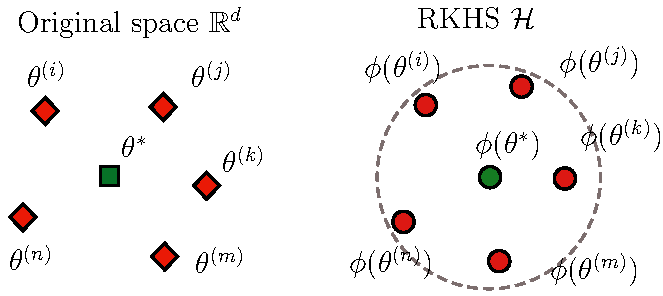
\includegraphics[width=0.38\textwidth]{pre-image}\label{fig:pre-image}}
	\caption{An overview of kernel Adaptive MCMC transition and two inverse projection steps.}
\end{figure*}

\paragraph{Adaptive MCMC transition in RKHS}
\paragraph{Adaptive Tempering}

\subsection{Finding Pre-images in the Embedding Space}
Mapping $\phi(\theta^*)$ back to $\theta^*$ is referred to as \emph{pre-image} problem and formulated as:
\begin{equation}
	\theta^*=\arg\min_{\theta\in \mathbb{R}^{d}}\left\|\phi(\theta)-\phi(\theta^*)\right\|^2_{\mathcal{H}}
	\label{equ:pre-image}
\end{equation}
In general, (\ref{equ:pre-image}) is a non-convex minimization problem and therefore difficult to solve. Sejdinovic et al. (2014) \cite{MCMC_Kameleon} employed a simple yet rather 
unreliable short-cut to get an approximate solution: by moving a single descent step along the gradient of (\ref{equ:pre-image}). 
Although by doing this they can obtain a simple multivariate Gaussian in $\mathbb{R}^d$ (\ref{equ:proposal_Kameleon}), yet it can only be applied on differentiable kernels. 
Here, instead, we put forward a new and more general method for pre-images by exploiting the \emph{topology consistence} within a small local area between the original space and the 
Hilbert space. Basically, we assume that  within a small area the spatial configuration of points will not change too much after being projected into a Hilbert 
space (Figure \ref{fig:pre-image}). The method is quite simple as follows: 
\begin{equation}
	\theta^*=\sum_{u=1:\phi(z^{(u)})\in\mathbf{N}(\phi(\theta^*))}^{U} w^{(u)} z^{(u)} \left/ \sum_{u=1:\phi(z^{(u)})\in\mathbf{N}(\phi(\theta^*))}^{U} w^{(u)}\right.
\end{equation}
where $\mathbf{N}(\phi(\theta^*))$ denotes the neighbourhood of $\phi(\theta^*)$ in $\mathcal{H}$ and it was obtained by ranking values of 
$w^{(u)}=K(z^{(u)}, \theta^*)$  and taking the top $U$ ones.   
\subsection{Projection onto $\mathcal{M}$}
After begin projected to the embedding space, $\theta^*$ usually still lays outside of $\mathcal{M}$. Therefore, we need one extra projection $\mathbf{P}$ to map $\theta^*$ onto $\mathcal{M}$:
\begin{equation}
	\mathbf{P}(\theta^*)=\arg\min_{\theta\in\mathcal{M}}\left\|\theta-\theta^* \right\|^2 
\end{equation}
In general, to solve the above convex objective function, we can resort to numerical optimization methods on 
Riemannnian manifolds \cite{optimization_manifold}. 
In our experiments, $SO(3)$ manifold and Stiefel manifold are considered,  projection on them actually can be more easily computed. 
\begin{theorem}
	Given an arbitrary matrix $A\in\mathbb{R}^{p\times r}$, its projection onto the Stiefel manifold $St(r,p)$ is:
	\begin{equation}
		\mathbf{P}_{St} (A)=UV^{\top}, \quad  \text{where U and  V are left and right eigenvectors of B respectively}. 
	\end{equation}
\end{theorem}
\begin{theorem}
	Given an arbitrary matrix $B\in\mathbb{R}^{p\times p}$, its projection onto $SO(3)$ manifold is:
	\begin{equation}
		\mathbf{P}_{SO} (B)=UV^{\top}, \quad  \text{where U and  V are left and right eigenvectors of A respectively}. 
	\end{equation}
\end{theorem}

\begin{proof}
	See \cite{projection_M}. 
\end{proof}

\subsection{A Finite-time Performance Guarantee}
\begin{corollary}
	Let Assumption \ref{assumption:basics} and the conditions in Theorem \ref{theorem:SA} hold, when $J$ satisfies the lower bound defined in (\ref{equ:J_bound}),
	\label{corollary:new}
\end{corollary}
\begin{equation}
	P_{\theta_{k(J)}}(\Theta(\epsilon,\alpha))\geq \left[\sigma-\eta (N^{\frac{3}{4}}+(N+1)^{\frac{3}{4}})\mathbf{Std}[\pi(\cdot;J,\delta)]\right] \cdot \text{erf}(\frac{\eta}{\sqrt{2}})^2
\label{equ:new_bound}
\end{equation}
where $\eta\in\mathbb{R}^+$, $N$ is the size of the particle set, $\text{erf}(\cdot)$ denotes \emph{Gauss error function} and $\mathbf{Std}[\tau]$ is the standard deviation of a distribution $\tau$.    
\begin{proof}
	See Appendix
\end{proof}
We can see (\ref{equ:new_bound}) provides a more informative bound than (\ref{equ:prob_bound}). In particular, (\ref{equ:new_bound}) explicitly 
invovles $\mathbf{Std}[\pi(\cdot;J,\delta)]$ , which is an important factor to analysis. For instance, if $f$ is a unimodal function and $J$ is 
sufficiently large, $\mathbf{Std}[\pi(\cdot;J,\delta)]$ will be quite close to 0.  
\begin{corollary}
	Let Assumption \ref{assumption:basics} and the conditions in Theorem \ref{theorem:SA} hold, when $J$ satisfies the lower bound defined in (\ref{equ:J_bound}),
	\label{corollary:set_bound}
\end{corollary} 
\begin{equation}
	P_{\theta_{k(J)}}(\Theta(\epsilon,\alpha)\in \mathcal{S})\geq 1-\left\{1-\left[\sigma-\eta (N^{\frac{3}{4}}+(N+1)^{\frac{3}{4}})\mathbf{Std}[\pi(\cdot;J,\delta)]\right] \cdot \text{erf}(\frac{\eta}{\sqrt{2}})^2\right\}^N
\end{equation}
\begin{proof} Since particles in KASMC are not independent, instead,    
	\begin{equation}
		P_{\theta_{k(J)}}(\Theta(\epsilon,\alpha)\in \mathcal{S})=1-P(\forall \theta^{(n)} \in \mathcal{S}, \theta^{(n)}\neq \Theta(\epsilon,\alpha))\geq 1-[1-P_{\theta_{k(J)}}(\Theta(\epsilon,\alpha)]^N
	\end{equation}	
\end{proof}
\newpage 
\section{Experiments}
Two experiments were conducted for practical tasks: finding optimal rotation and finding optimal subspace. For comparison, besides KASMC, we also tested 
other four algorithms: \emph{i}.$N$ independent simulated annealing (N-SA); \emph{ii}.SMC; \emph{iii}.Adaptive SMC (ASMC); \emph{iv}.KASMC with one gradient move for computing pre-images (KASMC-P). 
$N$ in N-SA is set to be equivalent to the number of particles in SMCs. Since there is no adaptive tempering in N-SA and SMC, their temperature sequences are set by using  
popular logarithmic schedule $J_k=\lfloor \log k \rfloor+1$ until it hits the target $J$. Except  pre-image computation step, other components in KASMC-P and KASMC are set up in the same way. In addition, the same projection 
procedure onto manifolds are used in all five algorithms.

\subsection{Rotation Optimization on $SO(3)$ Manifold} 
The first experiment is for 3D point cloud registration, which is difficult without prior knowledge of correspondence. 
Two point clouds $X$ and $Y$ were generated by first sampling a point set from a 3D mesh file and then applying two different 3D transformations on it. 
Since there is no noisy, translation  can be ignored by simply shifting the centers of two point clouds to the origin.     
Then the objective function on only rotation can be defined as:
\begin{equation}
	f(\theta)=\frac{1}{1+\mathcal{L}(\theta)} \quad \quad  \mathcal{L}(\theta)=\sum_{m=1}^M (x^{(c(m))}-\theta y^{(m)}), \quad \quad \theta\in SO(3)
\end{equation}
where $M=|Y|$, $\{x^{(c(m))},y^{(m)}\}$ is a pair of matching points in $X$ and $Y$ respectively, and the matching of $\theta y^{(m)}$ is found by searching a point in $X$, $x^{(c(m))}$, 
which is closest to it.  
Obviously, $f$ is a black-box function on $SO(3)$ and bounded within the range $(0,1]$. 

%\begin{figure}[t]
%	\centering
%	\subfigure[]{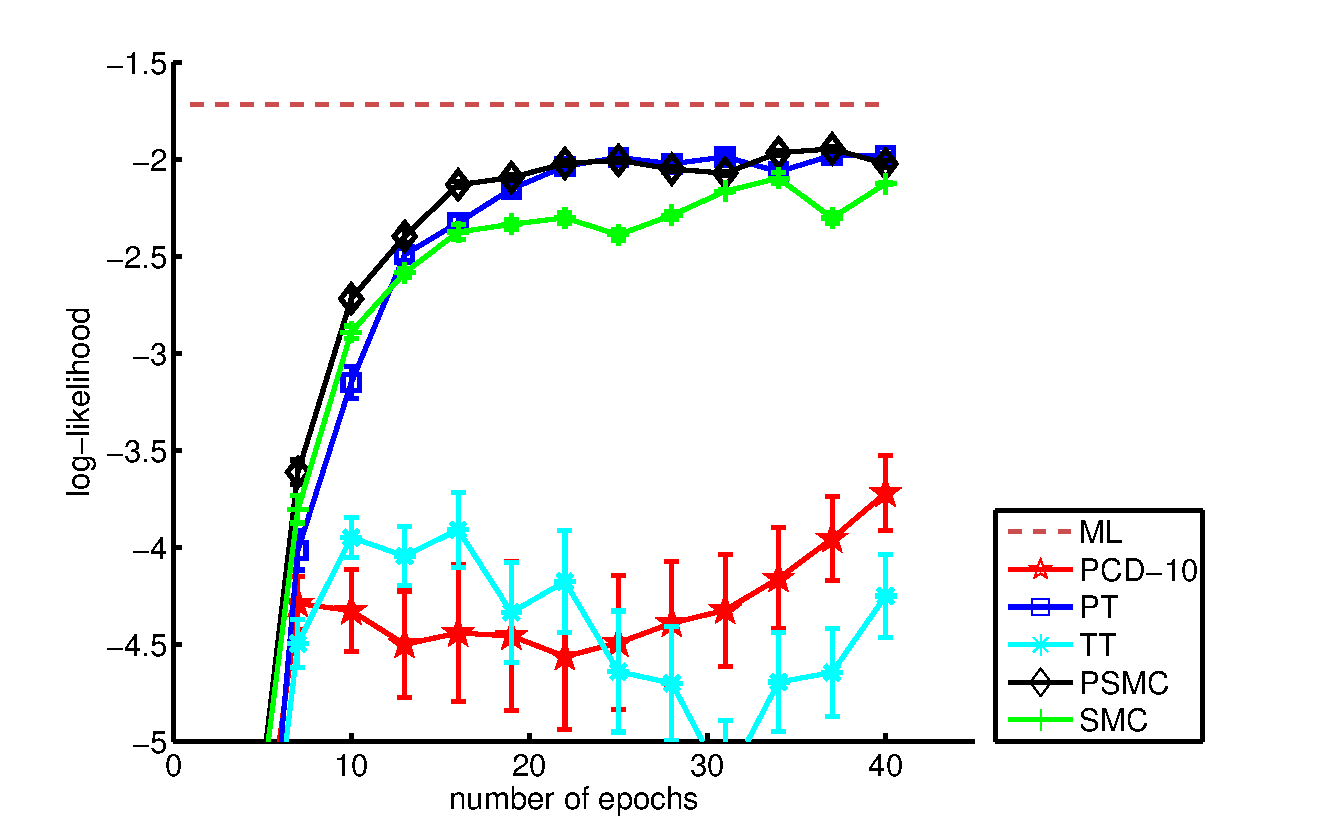
\includegraphics[width=.45\textwidth]{comparison_2}}
%	\subfigure[]{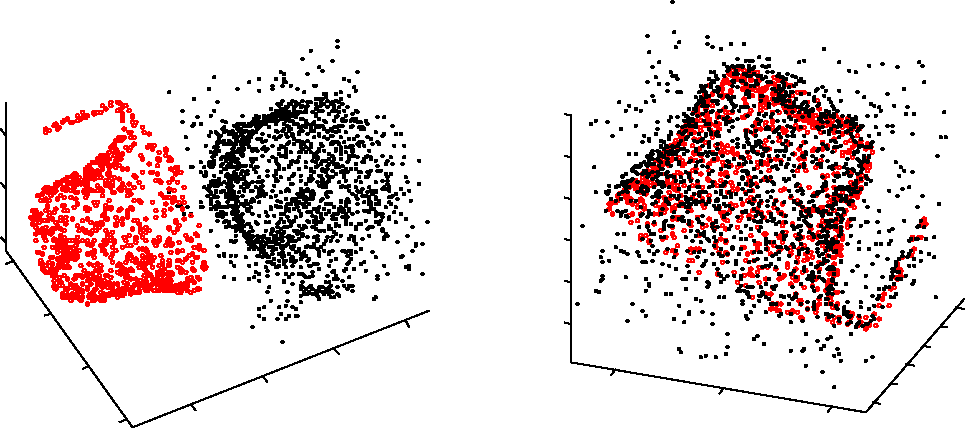
\includegraphics[width=.45\textwidth]{aligned}}
%	\caption{Image 1}
%\end{figure}

\begin{figure}[t]
	\centering
  \begin{minipage}[b]{0.48\linewidth}
      \subfigure[]{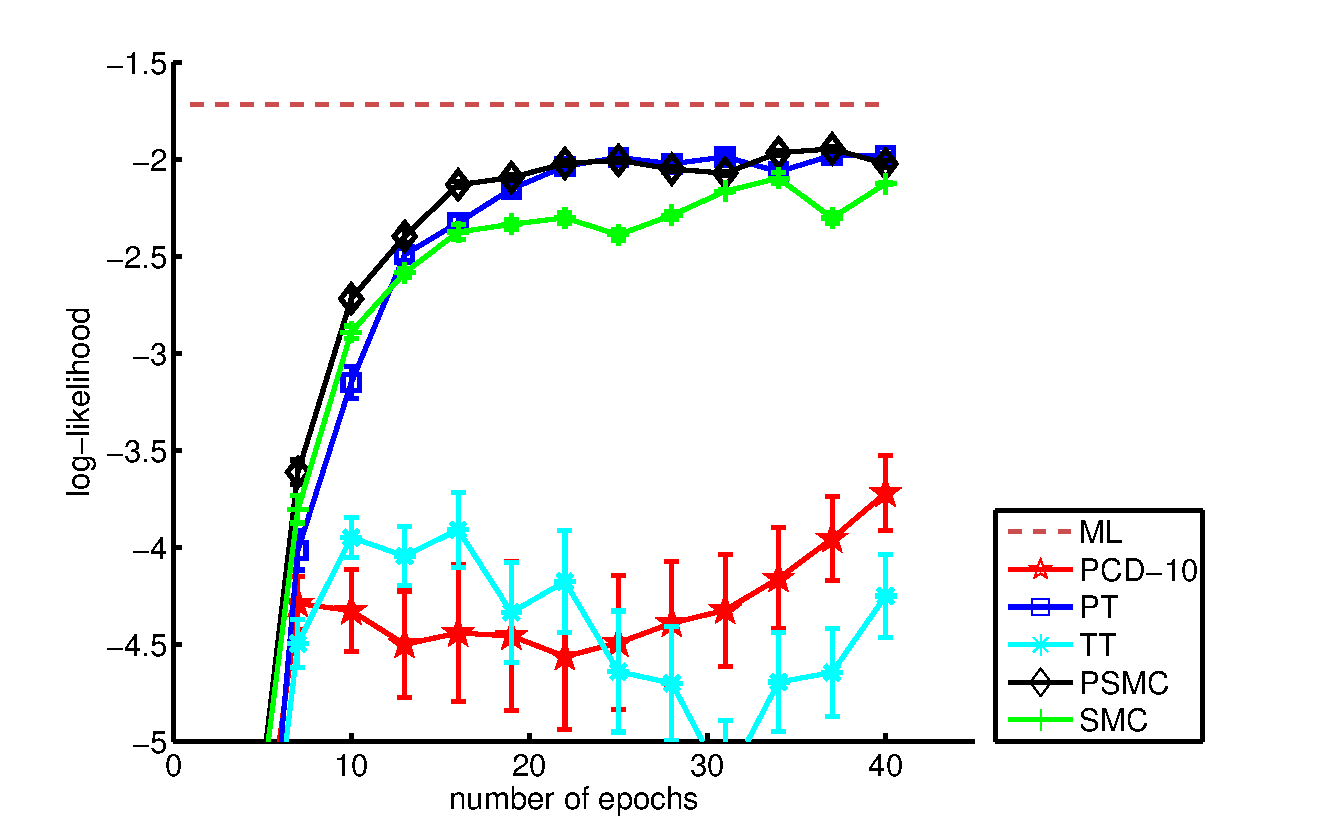
\includegraphics[width=.9\textwidth]{comparison_2}}
  \end{minipage}
  \begin{minipage}[b]{0.48\linewidth}
      \subfigure[]{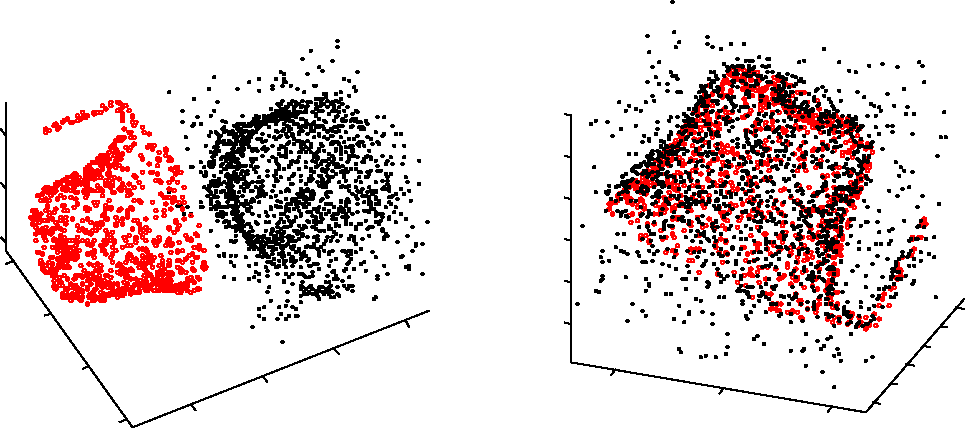
\includegraphics[width=.9\textwidth]{aligned}}
  \end{minipage}

  \begin{minipage}[b]{0.48\linewidth}
	  \subfigure[]{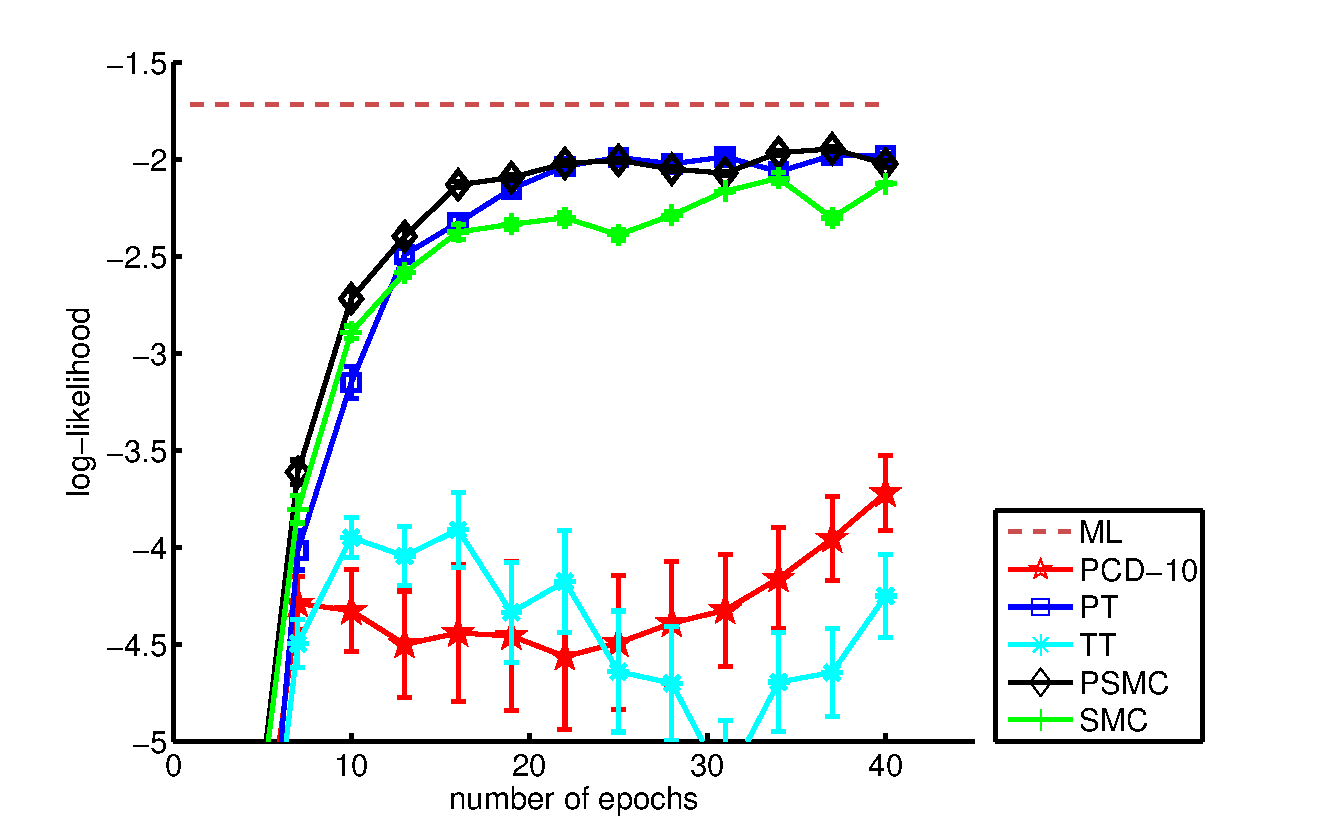
\includegraphics[width=.9\textwidth]{comparison_2}}
  \end{minipage} 
  \begin{minipage}[b]{0.48\linewidth}
	  \subfigure[]{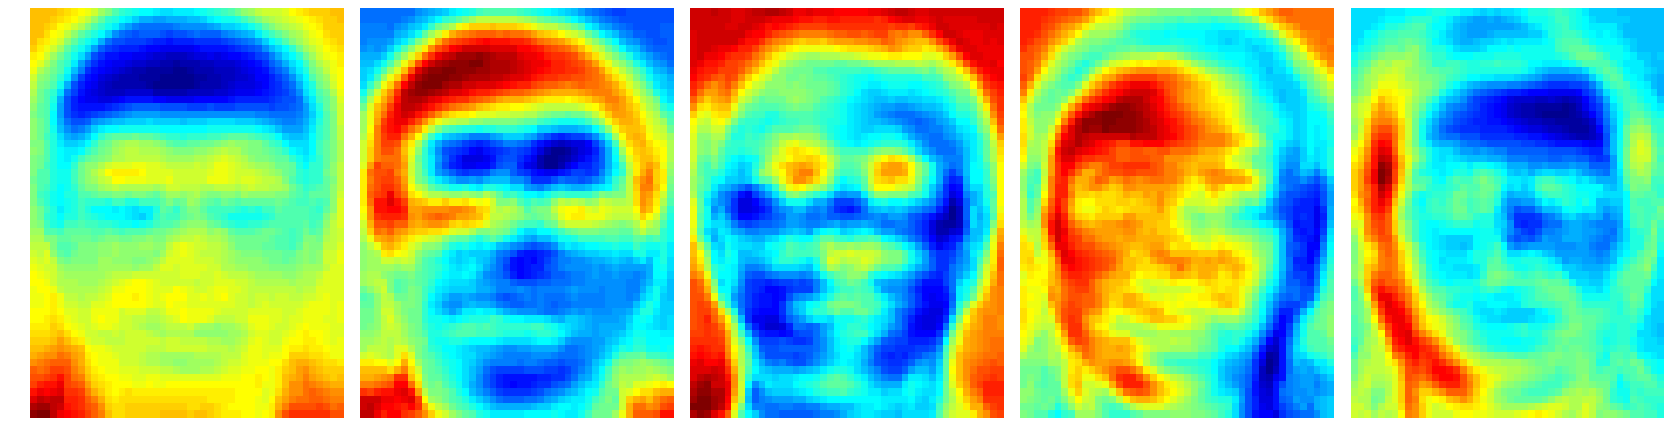
\includegraphics[width=.9\textwidth]{PCA_results}\label{fig:discriminative_bases}}
	  \subfigure[]{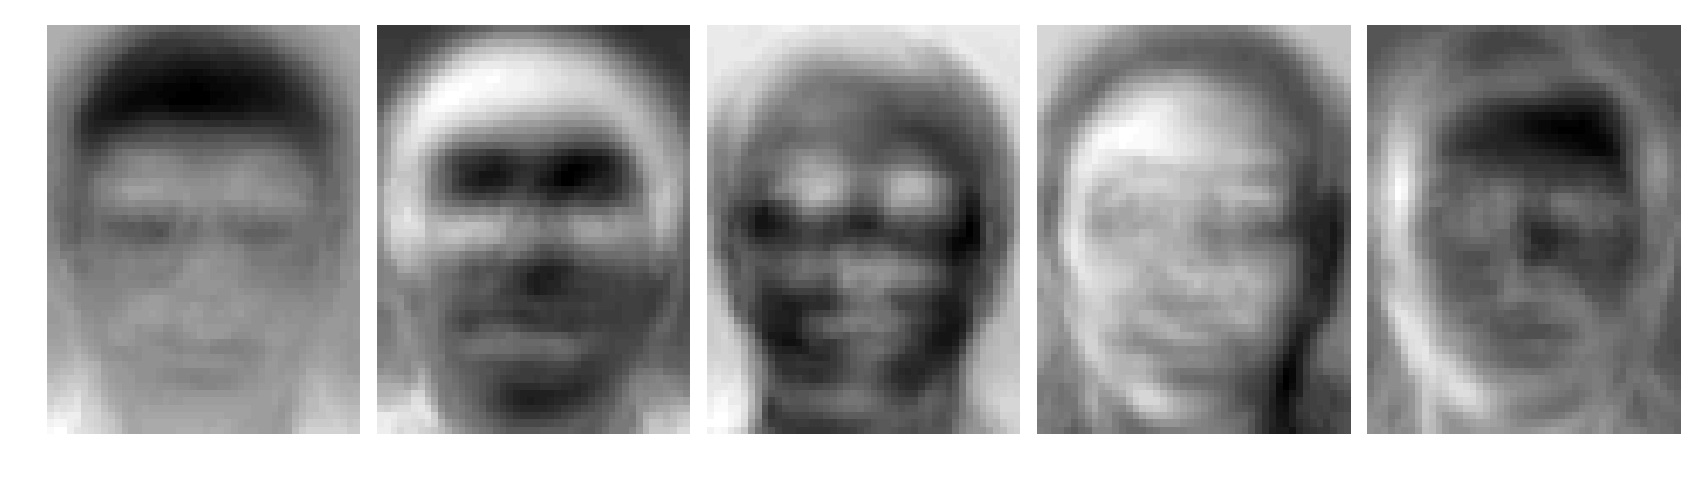
\includegraphics[width=.9\textwidth]{PCA_results_gray} \label{fig:PCA_results}}
  \end{minipage}
  \caption{(a) (c) Performance comparison of five optimization algorithms in the rotation optimization experiment and subspace optimization experiment respectively. 
  (b) Optimal rotation found by KASMC for 3D registration. (d) 5 bases of the optimal subspace. (e) 5 bases computed using PCA.}
\end{figure}

\subsection{Subspace Optimization on Stiefel Manifold}
The second experiment is for wearing-glass classification (\emph{i.e.} determine whether a face image has glass), and the target is to find optimal subspace of human faces for minimizing 
misclassification loss. For simplicity, we used \emph{K-nearest-neighbour} (KNN) for classification.  
We used images from the \emph{ORL face database} \cite{orl_database} and shrank them to $\frac{1}{4}$ of the original size (\emph{i.e.} $28\times 23$). 
Half of them were used for training and the other half for testing.  
Here our interest is a $5$ dimensional subspace, therefore, the search space is a Stiefel manifold $St(5,d=28\times 23)$.   
\begin{equation}
	f(\theta)=\frac{1}{1+\mathcal{L}(\theta)} \quad \quad  \mathcal{L}(\theta)=\text{misclassification error}, \quad \quad \theta\in St(5,d)
\end{equation}
Obviously, $f$ is a black-box function on $St(5,d)$. Assume there exist $M$ test instances then $f(\theta)\in[\frac{1}{M+1},1]$. 
Furthermore, we visualize 5 discriminative bases in Figure \ref{fig:discriminative_bases}. We can see that all 5 bases focus around eyes, which differ very much from the ones from 
using PCA (Figure \ref{fig:PCA_results}). 

\section{Conclusion}
A new stochastic optimization method was presented for black-box functions on Riemannian manifolds.
Many state-of-the-art studies were exploited. The proposed KASMC optimizer outperforms classic 
methods in both effectiveness and efficiency. As a possible future work direction, we are going to investigate 
how KASMC can be combined other strategies: \emph{e.g.} Bayesian optimization or optimistic optimization.    


\section*{Appendix}
Based on Theorem \ref{theorem:CLT},  given a particle set $\mathcal{S}=\{\theta^{(n)}\}_{n=1}^N, N\geq 30$, when the inverse temperature 
reaches $J$, 
\begin{equation}
	\forall \mathcal{S}\subseteq \mathcal{M}, \quad\quad \frac{1}{N} \sum_{n=1:\theta^{(n)}\in\mathcal{M}}^N(P_{\theta_{k(J)}}(\theta^{(n)})-\pi(\theta^{(n)};J,\delta)) \sim \mathcal{N}(0, \Sigma)
\end{equation}
where $\Sigma= N^{-\frac{1}{2}}\mathbf{Var}[\pi(\cdot;J,\delta)]$. By using \emph{cumulative density function} (CDF) , we have $P(E)=\text{erf}\left(\frac{\eta}{\sqrt{2}}\right)$, where $E$ denotes the following event:
\begin{equation}
	-\eta N^{-\frac{1}{4}}\mathbf{Std}[\pi(\cdot;J,\delta)]\leq \frac{1}{N}\sum_{n=1:\theta^{(n)}\in\mathcal{M}}^N (P_{\theta_{k(J)}}(\theta^{(n)})-\pi(\theta^{(n)};J,\delta))\leq \eta N^{-\frac{1}{4}}\mathbf{Std}[\pi(\cdot;J,\delta)] 
\end{equation}
\begin{equation}
	\Longleftrightarrow  -\eta N^{\frac{3}{4}}\mathbf{Std}[\pi(\cdot;J,\delta)]\leq \sum_{n=1:\theta^{(n)}\in\mathcal{M}}^N (P_{\theta_{k(J)}}(\theta^{(n)})-\pi(\theta^{(n)};J,\delta))\leq \eta N^{\frac{3}{4}}\mathbf{Std}[\pi(\cdot;J,\delta)] 
\label{equ:sigma_bound}
\end{equation}
With the same probability ($P(E^\dagger)=\text{erf}\left(\frac{\eta}{\sqrt{2}}\right))$, (\ref{equ:sigma_bound}) also holds for $\mathcal{S}^{\dagger}=\mathcal{S}\cup \theta^\dagger$, where $\theta^\dagger \in \mathcal{M}-\mathcal{S}$:
\begin{equation}
	-\eta (N+1)^{\frac{3}{4}}\mathbf{Std}[\pi(\cdot;J,\delta)]\leq \sum_{n=1:\theta^{(n)}\in\mathcal{S}\cup \theta^\dagger}^{N+1} (P_{\theta_{k(J)}}(\theta^{(n)})-\pi(\theta^{(n)};J,\delta))\leq \eta (N+1)^{\frac{3}{4}}\mathbf{Std}[\pi(\cdot;J,\delta)] 
\end{equation}
therefore, with probability $P(E^*)=\text{erf}(\frac{\eta}{\sqrt{2}})^2$, where $E^*$ denotes the following event: 
\begin{equation}
	\left|P_{\theta_{k(J)}}(\theta^\dagger)-\pi(\theta^\dagger;J,\delta)\right|\leq \eta (N^{\frac{3}{4}}+(N+1)^{\frac{3}{4}})\mathbf{Std}[\pi(\cdot;J,\delta)]
\end{equation}
Since $\mathcal{S}$ and therefore $\theta^{\dagger}$ are arbitrary, $E^*$ is equivalent to
\begin{equation}
	\sup_{\theta\in\mathcal{M}}\left|P_{\theta_{k(J)}}(\theta)-\pi(\theta;J,\delta)\right|\leq \eta (N^{\frac{3}{4}}+(N+1)^{\frac{3}{4}})\mathbf{Std}[\pi(\cdot;J,\delta)]
\end{equation}
%\begin{equation}
%	\Longleftrightarrow \int \left|(P_{\theta_{k(J)}}(\theta)-\pi(\theta;J,\delta))\right| d\theta \leq 2 \cdot 3 N^{-\frac{1}{4}}\mathbf{Std}(\pi(\cdot;J,\delta))
%\end{equation}
%\begin{equation}
%	\Longleftrightarrow ||(P_{\theta_{k(J)}}(\theta)-\pi(\theta;J,\delta))||_{TV}=\frac{1}{2} \int \left|(P_{\theta_{k(J)}}(\theta)-\pi(\theta;J,\delta))\right| d\theta \leq 3 N^{-\frac{1}{4}}\mathbf{Std}(\pi(\cdot;J,\delta))
%\end{equation}
Therefore, when $J$ satisfies the lower bound defined in (\ref{equ:J_bound}),   
\begin{equation}
	P_{\theta_{k(J)}}(\Theta(\epsilon,\alpha))\geq \left[\sigma-\eta (N^{\frac{3}{4}}+(N+1)^{\frac{3}{4}})\mathbf{Std}[\pi(\cdot;J,\delta)]\right] \cdot\text{erf}(\frac{\eta}{\sqrt{2}})^2
\end{equation}
 
%\subsection*{Acknowledgements}
%Use unnumbered third level headings for the acknowledgements title.
%All acknowledgements go at the end of the paper.



\newpage
\section*{Acknowledgement}
	The research leading to these results has received funding
from the European Community's Seventh Framework Programme
FP7/2007-2013 (Specific Programme Cooperation, Theme 3, Information
and Communication Technologies) under grant agreement no. 270273,
Xperience.


\bibliographystyle{abbrv}
\footnotesize 
\bibliography{refs}

\end{document}
